\section{Data Mining and Frequent Itemset Mining}
As already introduced, data mining represents a family of tools and techniques aimed at extracting usable and effective knowledge from collections of data. It is possible to distinguish 3 main groups of techniques:
\begin{itemize}
\item Unsupervised Learning (Clustering)~\cite{Xu_2005SurveyClustering}
\item Supervised Learning~\cite{AggarwalBookClassification}
\item Frequent Itemset Mining and Correlation Discovery~\cite{Han_2007SurveyFIM}
\end{itemize}

The goal of clustering and, more in general, unsupervised learning is to discover hidden structures in unlabeled data. Specifically, the aim of this set of techniques is grouping sets of objects in such a way that objects grouped together (in the same cluster) are more similar to each other than to those in other groups (clusters). The greater the homogeneity inside a group and the dissimilarity among different groups, the better the clustering results can be considered. The division into groups can be seen as an attempt to get the natural structure of the data.

Supervised Learning, instead, starting from a set of labeled input data, aims at building a predictive model from it. This model, which is an inferred function, should approximate the distribution of the input dataset, called training set, with respect to the class labels. The built model is then used to classify new unlabeled samples. 
%A very widespread trend in the age of big data and distributed computing, is to build many simple sub-models and then smartly merge them into a global predictive model.

Frequent Itemset Mining is an exploratory data analysis method used to discover frequent co-occurrence among the items of a transactional dataset (attribute-value pairs). The support of an itemset, a set of items, is the number of transactions in which it appears. A set of items is considered frequent if its support is over a user-provided frequency threshold (minimum support). 
Frequent Itemsets are very used also to summarize large collection of data since they output the most frequent patterns, which can be interpret as the most representative \cite{glatz2014visualizing}. In a similar way, they can be leveraged to highlight patterns which do not respect the most common trend \cite{cagliero2014infrequent},\cite{gupta2011minimally}. They can hide interesting outliers which could worth to be investigated and deepened \cite{paredes2012practical},\cite{brauckhoff2012anomaly}.
Frequent itemsets are often used as input to Association rules mining, a method to discover interesting relations between objects. They were first introduced analyzing retail transactions data from supermarkets. Each rule is organized on two members, respectively called antecedent and consequent. The rule concept is very straightforward and an example rule is: $\{bread, butter\} \rightarrow \{milk\}$. This rule means that customers who buy bread and butter usually buy also milk. Of course, the rules should be considered statistically significant just if supported by a sufficient support and confidence (i.e. how often the rule has been found to be true).
Association rules and, in general, the extracted knowledge in terms of correlations, could be considered very valuable information. For instance, a whole category of classifier or recommendation systems are based on rules \cite{LiuHM98},\cite{Venturini2016}.


In the following Subsection, a preliminary background, useful to better understands the content of this work, will be introduced. 

\subsection{Frequent Itemset Mining - Preliminaries}\label{itemset_preliminaries}

%
%\begin{figure}[!t]
%%\renewcommand{\arraystretch}{1.3}
%%\centerline
%{\subfloat[Horizontal representation of $\mathcal{D}$]{
%\label{back_horizontalexampledataset}
%\begin{tabular}{|c|l|}
%\hline
%\multicolumn{2}{|c|}{$\mathcal{D}$}\\
%\hline
%\hline
%	tid & items \\
%\hline
%	1 & a,b,c,l,o,s,v \\
%\hline
%	2 & a,d,e,h,l,p,r,v \\
%\hline
%	3 & a,c,e,h,o,q,t,v \\
%\hline
%	4 & a,f,v \\
%\hline
%	5 & a,b,d,f,g,l,q,s,t \\
%\hline
%\end{tabular}}}%
%\hfil
%{\subfloat[Transposed representation of $\mathcal{D}$]{
%\label{back_TTexampledataset}
%\begin{tabular}{|c|l|}
%\hline
%\multicolumn{2}{|c|}{$TT$}\\
%\hline
%\hline
%	item & tidlist \\ \hline
%	a & 1,2,3,4,5 \\ \hline
%	b & 1,5 \\ \hline
%	c & 1,3 \\ \hline
%	d & 2,5 \\ \hline
%	e & 2,3 \\ \hline
%	f & 4,5 \\ \hline
%	g & 5 \\ \hline
%	h & 2,3 \\ \hline
%	l & 1,2,5 \\ \hline
%	o & 1,3 \\ \hline
%	p & 2 \\ \hline
%	q & 3,5 \\ \hline
%	r & 2 \\ \hline
%	s & 1,5 \\ \hline
%	t & 3,5 \\ \hline
%	v & 1,2,3,4 \\ \hline
%\end{tabular}}}%
%\hfil
%{\subfloat[Transposed representation of $\mathcal{D}$]{
%\label{back_TTexampledataset}
%\begin{tabular}{|c|l|}
%\hline
%\multicolumn{2}{|c|}{$TT$}\\
%\hline
%\hline
%	item & tidlist \\ \hline
%	a & 1,2,3,4,5 \\ \hline
%	b & 1,5 \\ \hline
%	c & 1,3 \\ \hline
%	d & 2,5 \\ \hline
%	e & 2,3 \\ \hline
%	f & 4,5 \\ \hline
%	g & 5 \\ \hline
%	h & 2,3 \\ \hline
%	l & 1,2,5 \\ \hline
%	o & 1,3 \\ \hline
%	p & 2 \\ \hline
%	q & 3,5 \\ \hline
%	r & 2 \\ \hline
%	s & 1,5 \\ \hline
%	t & 3,5 \\ \hline
%	v & 1,2,3,4 \\ \hline
%\end{tabular}}}%
%%\hfil
%%{\subfloat[$TT|_{\{2,3\}}$: example of con\-di\-tio\-nal
%%tran\-spo\-sed table]{
%%\label{conditionalexampledataset}
%%\begin{tabular}{|l|l|}
%%\hline
%%\multicolumn{2}{|c|}{$TT|_{\{2,3\}}$}\\
%%\hline
%%\hline
%%item & tidlist \\ \hline
%%a &4,5 \\ \hline
%%e & - \\ \hline
%%h & -\\ \hline
%%v &4 \\ \hline
%%\end{tabular}}}%
%\caption{Running example dataset $\mathcal{D}$}
%\label{back_exampledataset}
%\end{figure}


\begin{figure}[!t]
%\renewcommand{\arraystretch}{1.3}
%\centerline
{\subfloat[Horizontal representation of $\mathcal{D}$]{
\label{back_horizontalexampledataset}
\begin{tabular}{|c|l|}
\hline
\multicolumn{2}{|c|}{$\mathcal{D}$}\\
\hline
\hline
	tid & items \\
\hline
	1 &	a b c d \\
\hline
2 &	a c d e\\
\hline
	3 &b c d e\\
\hline
4 &	a d e \\

\hline
\end{tabular}}}%
\hfil
{\subfloat[Transposed representation of $\mathcal{D}$]{
\label{back_TTexampledataset}
\begin{tabular}{|c|l|}

\hline
\multicolumn{2}{|c|}{$TT$}\\
\hline
\hline
	item & tidlist \\ \hline
	a & 1,2,4 \\ \hline
	b & 1,3 \\ \hline
	c & 1,2,3 \\ \hline
	d & 1,2,3,4 \\ \hline
	e & 2,3,4 \\ \hline
\end{tabular}}}%
\hfil
{\subfloat[Frequent itemset extracted from $\mathcal{D}$ with a minsup=2 ]{
\label{back_frequent}
\begin{tabular}{|c|l|}
\hline
\multicolumn{2}{|c|}{Frequent Itemsets}\\
\hline
\hline
itemsets & Support \\
\hline
a & 3\\
\hline
b & 2 \\
\hline
c & 3\\
\hline
d & 4\\
\hline
e& 3 \\ 
\hline
	a c & 2\\
\hline
	a d & 3\\
\hline
	a e & 2\\
\hline
	b c & 2\\
\hline
b d & 2\\
\hline
	c d & 3\\
\hline
	c e & 2\\
\hline
	d e & 3\\
\hline
a c d & 2\\
\hline
a d e& 2\\
\hline
b c d & 2\\
\hline
c d e & 2\\
\hline
\end{tabular}}}%
%\hfil
%{\subfloat[$TT|_{\{2,3\}}$: example of con\-di\-tio\-nal
%tran\-spo\-sed table]{
%\label{conditionalexampledataset}
%\begin{tabular}{|l|l|}
%\hline
%\multicolumn{2}{|c|}{$TT|_{\{2,3\}}$}\\
%\hline
%\hline
%item & tidlist \\ \hline
%a &4,5 \\ \hline
%e & - \\ \hline
%h & -\\ \hline
%v &4 \\ \hline
%\end{tabular}}}%
\caption{Running example dataset $\mathcal{D}$}
\label{back_exampledataset}
\end{figure}

Let $\mathcal{I}$ be a set of items. A transactional dataset $\mathcal{D}$
consists of a set of transactions $\{t_1, \dots, t_n\}$,
where each transaction $t_i\in \mathcal{D}$ is a set of items (i.e.,
$t_i\subseteq \mathcal{I}$)
and it is identified by a transaction identifier ($tid_i$).
Figure~\ref{back_horizontalexampledataset} reports an example of a transactional
dataset with 4 transactions.

An itemset $I$ is defined as a set of items (i.e., $I\subseteq\mathcal{I}$) and
it is characterized by a tidlist and a support value.
The tidlist of an itemset $I$, denoted by $tidlist(I)$, is defined as the set of
tids of the transactions in $\mathcal{D}$ containing $I$,
while the support of $I$ in $\mathcal{D}$, denoted by $sup(I)$, is defined as
the ratio between the number of transactions in $\mathcal{D}$ containing $I$
and the total number of transactions in $\mathcal{D}$ (i.e.,
$|tidlist(I)|/|\mathcal{D}|$).
For instance, the support of the itemset \textit{\{acd\}} in
the running example dataset $\mathcal{D}$ is 2/4 and its tidlist is $\{1,2\}$.
An itemset $I$ is considered frequent if its support is greater than a
user-provided minimum support threshold $minsup$. Figure~\ref{back_frequent}
reports the frequent itemset extracted from $\mathcal{D}$ with a minsup value equal to 2.

Given a transactional dataset $\mathcal{D}$ and a minimum support threshold
$minsup$, the Frequent Itemset Mining \cite{KumarBook} problem consists in
extracting the complete set of frequent itemsets from $\mathcal{D}$.
The dimension of the search space , which can be represented as a lattice with an empty set at the top and an itemset containing all the possible itemset at the bottom, scales exponentially with the number of items~\cite{goethals2003survey}.
In Figure~\ref{lattice}, it is shown the lattice related to our running example.


In this work, we focus also on a valuable subset of frequent itemsets called
frequent closed itemsets~\cite{Zaki_Carpenter}. Closed itemsets
allow representing the same information of traditional frequent itemsets in a
more compact form.
In addition, an item or itemset $I$ is closed in  $\mathcal{D}$ if there exists no superset that
has the same support count as  $I$.\\
For instance, in our running example, given a $minsup=2$, the itemset \textit{\{ac\}} is a frequent itemset (support=2), but it is not closed for the presence of the itemset \textit{\{acd\}} (support=2). 
% %If an itemset is frequent, all of its subsets are frequent for the
% \textit{monotonic property}.
% %For the same rule, if an items or an itemset is not frequent, none of its
% supersets are frequent. In addition, an items
% % or itemset $I$ is closed in  $\mathcal{D}$ if there exists no superset that
% has the same support count as  $I$.\\
\\
A transactional dataset can also be represented in a vertical format, which is
usually a more effective representation of the dataset when the average number
of items per transactions is orders of magnitudes larger than the number of
transactions.
In this representation, also called \textit{transposed table} $TT$, each
row consists of an item $i$ and its list of transactions, i.e.,
$tidlist(\{i\})$.
Figure~\ref{back_TTexampledataset} reports the transposed representation of the
running example reported in Figure~\ref{back_horizontalexampledataset}.

%Given a transposed table $TT$ and a tidlist $X$, the conditional transposed
%table of $TT$ on the tidlist $X$, denoted
%by $TT|_{X}$, is defined as a transposed table such that:
%(1) for each row $r_i\in TT$ such that $X\subseteq r_i.tidlist$ there exists one
%tuple $r_i^{\prime}\in TT|_{X}$ and
%(2) $r_i^{\prime}$ contains all tids in $r_i.tidlist$ whose tid is higher than
%any tid in $X$.
%For instance, consider the transposed table $TT$ reported in
%Figure~\ref{TTexampledataset}. The
%projection of $TT$ on the tidlist \textit{\{2,3\}} is the transposed table
%reported in Figure~\ref{conditionalexampledataset}.
%Each transposed table $TT|_{X}$ is associated with an itemset composed by the
%items in $TT|_{X}$.
%For instance, the itemset associated with $TT|_{\{2,3\}}$ is \textit{\{aehv\}}
%(see Figure~\ref{conditionalexampledataset}).


% %Given a row or a set of rows (in the sequel, \textit{row set}) $x$, $TT|_{x}$,
% is the projection of the whole vertical datasets on the row set x. Each
% transposed table is associated with an itemset composed of the items in the
% table. For each item, the associated tidlist is composed of the tids greater
% than any tid in the row set x. For instance, $TT|_{2,3}$ in tab 3 is the
% transposed table of the row set \textit{2,3} and it represents the itemset
% \textit{aehv}.

\begin{figure}[!t]
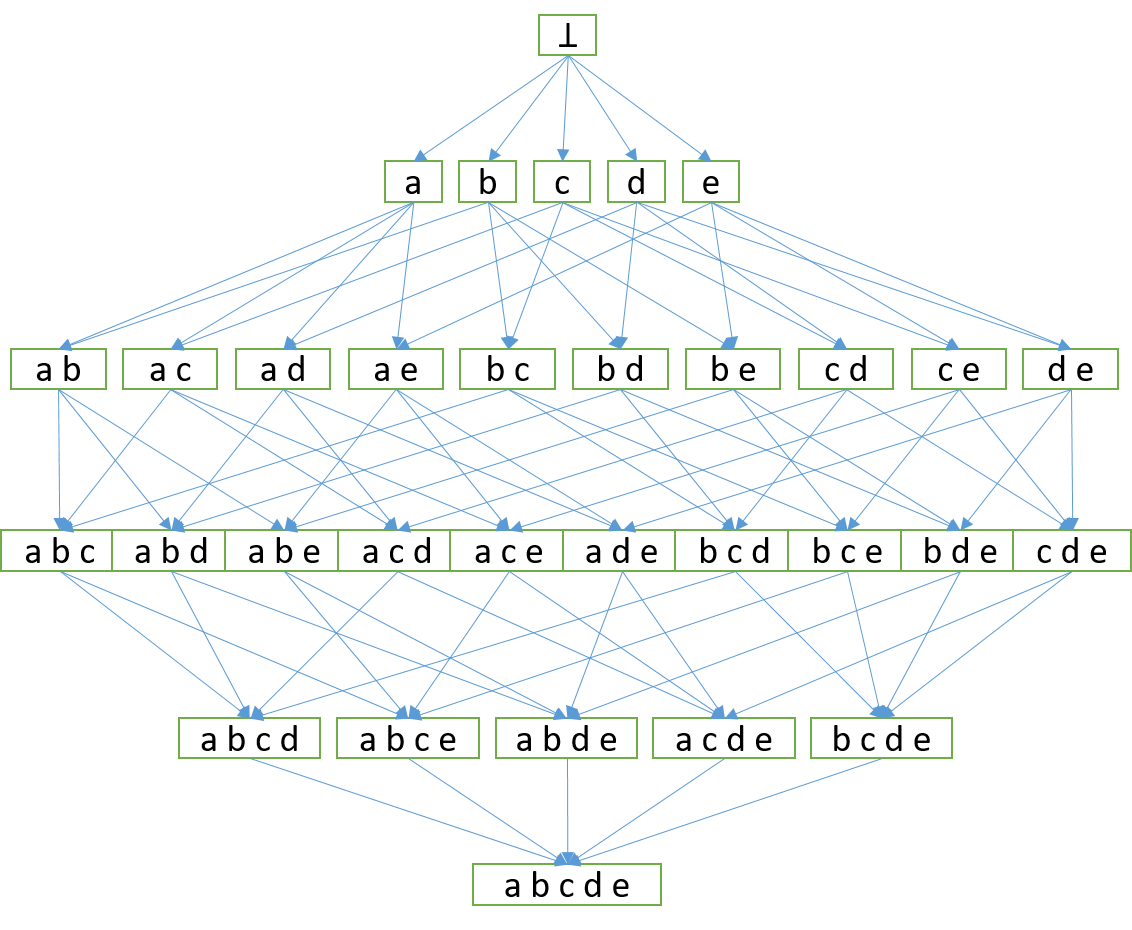
\includegraphics[width=5in]{chapters/lattices.png}
\caption{Lattice representing the search space of $\mathcal{D}$}
\label{lattice}
\end{figure}

\section{Big Data and Distributed Frameworks}
Today's shift towards horizontal scaling in hardware has highlighted the
need of distributed algorithms. Being able to analyze big data is a huge value from both an economic and social point of view. Unfortunately, traditional tools have demonstrated to be not reliable for dealing with such large amount of data.
%Starting from data storage, new solutions have to be developed to replace traditional relational database managements systems. 
% Thus, we
%are witnessing the explosion of distributed and parallel approaches, often
%accompanied with cloud-based services (e.g. Platform-as-a-Service
%tools)~\cite{ISPA13}.

Starting from data storage, new solutions had to be developed to replace traditional relational database managements systems. We have firstly witnessed the development of distributed file systems such as Google File System \cite{ghemawat2003google} and its derivative Hadoop Distributed File System~\cite{HDFS}. For the computational issues, already well-known parallel frameworks have shown their limitations due to fault tolerance and resiliency lacks. In the meanwhile, new processing models spread out. 
MapReduce~\cite{ArticoloMapReduceGoogle} is the most popular example of a generic batch-oriented distributed paradigm. With its reliable and fault-tolerant architecture, it allows to exploit the resources of more commodity machines (nodes). The ratio behind the spread of the paradigm is that 'shifts the computation to the data'.
In fact, taking advantage of the data locality, allowing the nodes to process just the shard of the data they store.

A MapReduce application consists of two main phases. In the first phase, called "map", each shard of the dataset is processed locally by each node of the commodity clusters, which output one or more key-values couples. Map results are exchanged among the cluster nodes and aggregate the tuples per key: this is the "shuffle" phase. This operation, which is very optimized, is one of the killer feature which a MapReduce-like algorithm should strongly exploit (it is also the unique communication among the nodes of the commodity cluster). Finally, the reduce phase is run for each unique keys and iterates through all the associated values.

Designed to cope with very large datasets, the Java-based framework Hadoop~\cite{HDFS} is the most widely adopted MapReduce implementation. It allows programmers not to concern to low level details and to focus just on the algorithm design.

However, Hadoop and MapReduce paradigm does not fit at all iterative processes. In this case, each iteration would require a complete read and transmission (shuffle phase) of the input dataset, which is critical when dealing with huge datasets. This issue motivated the development of a new in-memory distributed platform called Apache Spark~\cite{Zaharia_spark}. This framework, when possible, allows machines to cache data and intermediate results in memory, instead of reloading it from the disk at each iteration. Spark has also introduced a new type of data collection called RDD (Resilient Distributed Dataset). Every RDD modification is done just by the generation of another RDD, keeping trace of all the transformations in order to be able to regenerate data in case of failures. Furthermore, RDDs avoid on-disk materialization until not strictly mandatory, i.e. when an action requires a result to be returned to the driver program, saving resources in terms of communication and I/O costs. Spark supports both Graph-based and Streaming processes, demonstrating to be more flexible than Hadoop, still keeping full compatibility with the latter. 

Because of the winning features of Hadoop and Spark, testified by their spread in the academic environment, in this dissertation we will focus into these distributed frameworks, analyzing the best-in-class Hadoop and Spark-based works and utilizing their paradigm for further advancements of the state of the art.

However, Hadoop and Spark are
not the only frameworks supporting the parallelization of Data mining
algorithms. GraphLab~\cite{graphlab}, Google Pregel~\cite{pregel} and its
open-source counterpart Giraph~\cite{giraph} are fault-tolerant, graph-based
framework while SimSQL~\cite{simsql}, for instance, exploits an SQL-based
approach. Distributed systems are popular also because they became very easy to
use: as already stated, Message Passing Interface (MPI)~\cite{mpi}, one of the most adopted
framework in academic environment, works efficiently only on very low level
programming such as C.

\subsection{Hadoop and Spark Machine Learning Libraries}
In recent years the
success of these distributed platforms was supported by the introduction of open
source libraries of machine learning algorithms.
%These are very precious for the academic world
%since they allow researchers to save time for implementation or to use the
%algorithms as reference baseline for further optimizations.
% We strongly consider
%the presence of these libraries as a real advantage of a framework.
Mahout~\cite{Mahout} for Hadoop has represented one of the most popular
collection of Machine Learning algorithms, containing implementations in the
areas such as clustering, classification, recommendation systems, etc. All the
current implementations are based on Hadoop MapReduce.
MADlib~\cite{madlib},
instead, provides a SQL toolkit of algorithms that run over Hadoop. Finally,
MLLib~\cite{MLLib} is the Machine Learning library developed on Spark, and it is
rapidly growing up. MLLib allows researchers to exploit Spark special features
to implement all those applications that can benefit from them, e.g. fast
iterative procedures.

\section{Big Data and FIM (maybe should put this before 2.2)}
In this Section we will motivate the need of scalable frequent itemeset mining algorithms and their relations with input dataset size and
minimum support threshold. After that, the issues related to the problem statement will be discussed.

\textbf{Input size and minimum support value.} As already largely discussed, we are witnessing an explosive increasing of data availability. Process and support this extremely large amount of data is very challenging. Data mining algorithms, for their nature, as better detailed in the last part of this Section, are among the hardest processes to parallelize. Specifically, the parameters which most affect the mining are 2. The first, as predictable, is the input data size, while the second is the minimum support threshold. 

The first issue is already intuitive since a bigger data collection is harder to analyze. The problem is caused by the inner data structure (e.g., FP-tree \cite{Han00}, Enumeration Tree \cite{Zaki_Carpenter}, Prefix Tree \cite{Zaki97newalgorithms}, ...) leveraged by the algorithm itself to explore the search space. Larger datasets lead to larger data structures built by the algorithm itself. Larger data structures require large amount of memory and computational resources to be maintained and explored.

The second issue is related to minimum support threshold, which, in our problem, is directly mirrored to the targeted depth of the analysis. 
Even for datasets not belonging to big data environment, a very low support 
extraction could require huge amount of resources. 
The lower it is, the more challenging in terms of resource the mining will be. 
Therefore, it is likely to occur that frequent itemset miner is easily able to complete the itemsets extraction with a certain minimum support threshold, and running out of memory with the same input and a lower support. 
Even in this case, the motivations are related to the inner structure used by the algorithms to explore the search space~\cite{goethals2003survey}. A low minimum support threshold leads to a deeper exploration of the search space. For some algorithms like Apriori~\cite{Agr94}, it could lead to the generation and testing of all the possible combinations of the dataset items. The mining considers any possible items co-occurrency and it can happen that the output of the process exceeds the input data size (as clearly shown in Tables \ref{back_horizontalexampledataset} and \ref{back_frequent}). In addition, please note that the size and the complexity of these structure do not scale linear with the minimum support threshold \cite{KumarBook},~\cite{goethals2003survey}. For these reasons, this parameter is very important analyzing the performance of a frequent itemset mining algorithm. 







%
%
%
%
%
%
%
%\begin{table}[]
%
%\centering
%
%\caption{Example of frequent itemset mining with minsup of 50\% \label{toy_mining}}
%
%\begin{tabular}[t]{|c|c|}
%\hline
%\multicolumn{2}{|c|}{$\mathcal{D}$}\\
%\hline
%\hline
%tid & items \\
%\hline
%1 &	A B C D \\
%\hline
%2 &	A C D E\\
%\hline
%	3 &B C D E\\
%\hline
%4 &	A D E \\
%\hline
%
%\end{tabular}\qquad
%
%\begin{tabular}[t]{|c|l|}
%\hline
%\multicolumn{2}{|c|}{$TT$}\\
%\hline
%\hline
%	item & tidlist \\ \hline
%	A & 1,2,3,4,5 \\ \hline
%	B & 1,5 \\ \hline
%	C & 1,3 \\ \hline
%	D & 2,5 \\ \hline
%	E & 2,3 \\ \hline
%\end{tabular}\qquad
%\begin{tabular}[t]{|c|c|}
%\hline
%\multicolumn{2}{|c|}{Frequent Itemsets}\\
%\hline
%\hline
%itemsets & Support \\
%\hline
%A & 3\\
%\hline
%B & 2 \\
%\hline
%C & 3\\
%\hline
%D & 4\\
%\hline
%E& 3 \\ 
%\hline
%	A C & 2\\
%\hline
%	A D & 3\\
%\hline
%	A E & 2\\
%\hline
%	B C & 2\\
%\hline
%B D & 2\\
%\hline
%	C D & 3\\
%\hline
%	C E & 2\\
%\hline
%	D E & 3\\
%\hline
%A C D & 2\\
%\hline
%A D E& 2\\
%\hline
%B C D & 2\\
%\hline
%C D E & 2\\
%\hline
%\end{tabular}\qquad
%
%\end{table}
%




These two aspects are the most critical issues for itemset extraction. As we will see in Chapters \ref{survey} and \ref{pampa}, also input data distribution has an impact. For the sake of clarity, for the moment, we ignore this feature, which is very dependent on the algorithms nature. 
 

\textbf{Motivations.} Now, let us focus on the reasons behind the needs to mine huge datasets and/or extract itemsets with low minimum support thresholds. Focusing on the first aspect, the need of scalability in terms of input dataset size is an obvious consequence of the requirement to analyze huge data collections. Indeed, in big data analysis domain, frequent itemset mining is very useful tool. For instance, thinking about the summarization properties of frequent itemsets, we can assume that the larger is the dataset, the more essential would be its summarization.

%Now, let us focus on the need of lowering the minimum support threshold. 
As already mentioned, even low supports could represent very challenging mining processes. 
The reader could wonder about the need of such amount of frequent itemsets, given that, one of the most intuitive usage examples are related to data summarization.
However, in many applications, frequent pattern mining can be considered as a preprocessing than a final step. One of the most intuitive contexts is the "infrequent" itemset extraction and outlier detection algorithms \cite{cagliero2014infrequent},\cite{brauckhoff2012anomaly}. 
The need of a deep extraction is also motivated by the hitches to include any interestingness measures (apart from the support) into the extraction process. Hence, a very common behavior is to extract as many itemsets as possible and then apply any sort of interestingness filter. 
For instance, already in this dissertation, will be introduced a work, in which a special type of itemsets is mined from a set of frequent itemsets (see Chapter \ref{nemico} for further details).


\textbf{Challenges.} The parallelization of the mentioned data structures represents the main contribution behind the development of distributed and parallel frequent itemset mining algorithms. Like almost all the data mining tools, this technique, as already discussed, does not fit parallel and/or distributed implementations. 
%The first issue is related to the nature of the problem which assume a full knowledge of the data. 
In distributed an parallel domains, an ideal approach assumes to divide the problem into independent non-overlapping sub-problems, which can be assigned to commodity cluster nodes. In this way, (i) the resource are completely exploited and (ii) the communication costs, a concrete bottleneck in distributed environment, are reduced as much as possible.

In FIM environment, the task that should be parallelized is the search space exploration, which is done through ad-hoc data structures. As detailed in Chapters \ref{survey} and \ref{pampa}, all the distributed FIM algorithms smartly split and distribute the processing of these data structures, most of the them in "divide and conquer" fashion. This technique overcomes the main memory issues.
However, this split is often sub-optimal:
\begin{itemize}
\item First, in order to be independent for the mining task related to the respective algorithm, the set of resulting partitions could overlap each other (please note that the overlapping degree is dependent from the data distribution). Overlapping partitions entails that the global memory of the cluster should be larger than the already huge input data, storing redundant data \cite{Mahout},\cite{pampa_v1} which can lead to redundant and useless output \cite{bigfim},\cite{pampa_v1}. Furthermore, it increases the communication costs because more data have to be transmitted across the network.

\item In addition, in centralized algorithms, some pruning techniques are often used to limit the search space exploration, saving time and resources. Some of the challenges related to the parallelization of exploration task parallelization are the difficulties related to these pruning techniques, which assumes a state centralized memory. In \cite{pampa_v1}, we have addressed this issue, introducing a trade-off among the benefits related to a centralized memory ("state") and the ones related to the degree of parallelization (i.e. number of independent parallel tasks) (further details in Chapter \ref{pampa}).
\end{itemize}

These are the main challenges and the possible drawbacks related 
to a parallel implementation of frequent itemset mining algorithms. 
In the next Chapter we will evaluate how the best-in-class state of the art algorithms have addressed these questions. In Chapter \ref{pampa}, instead, we will introduce our solution concerning parallel \textit{high-dimensional} frequent pattern mining. 

